\section{Neural Networks}

Artificial neural networks are computational models for learning that have been around since at least the 1940's \cite{mcculloch1943logical, hebb2005organization}. Their popularity has waxed and waned over the last 7 decades, but in the last 10 years interest has grown dramatically as various computational components such as convolutional networks \cite{krizhevsky2012imagenet, kim2014convolutional, mnih2015human}, recurrent networks \cite{mikolov2010recurrent, graves2013generating, mnih2014recurrent}, and attention mechanisms \cite{gregor2015draw, vaswani2017attention, xu2015show} have shown impressive performance in a variety of classification, generation, and control tasks. The modern study of artificial neural networks is called {\em deep learning} to emphasize the use of deep networks with many layers of neurons. Deep learning has become a vast subfield of machine learning, with lengthy books and monographs dedicated to its study \cite{goodfellow2016deep, schmidhuber2015deep}. In this section we will briefly touch on some of the key ideas in deep learning that are used in the work found in Chapter 4.

\subsection{Overview and feedforward networks}

A neural network is a parametrized function $y = f(x;w)$ where $x$ is an input vector and $w$ is a vector of parameters for the function. What gives a neural network its distinctive characteristic is the modular and layered way in which its parameters are arranged in the computation process. A representation of a small neural network is shown below.

\begin{figure}
    \centering
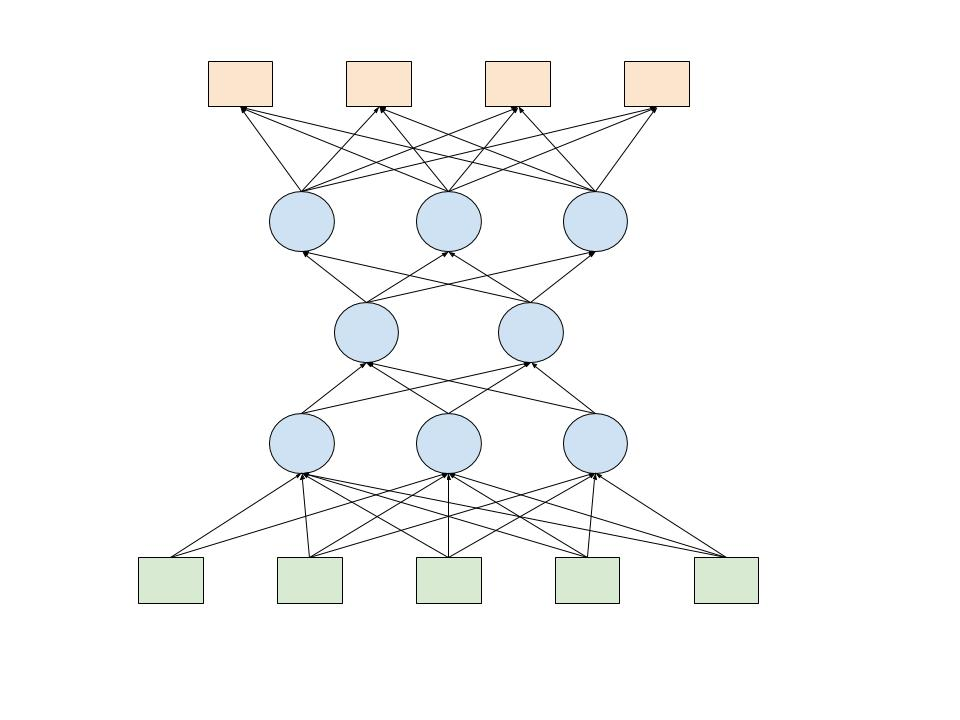
\includegraphics[scale=0.4]{images/Feedforward_network.jpg}
    \caption{A small neural network. The network has a 5 dimensional input, 4 dimensional output, and 3 hidden fully connected layers.}
    \label{fig:smallnn}
\end{figure}

The input vector $x$ is represented at the bottom by the 5 green blocks, indicating that the input is a 5-dimesional vector. The input vector undergoes 4 successive layers of computation. Each arrow in the diagram corresponds to a single parameter (also known as a {\em weight}) in the network. In the first layer, the input is transformed into a 3-dimensional vector. The result is then transformed into a 2-dimensional vector, a 3-dimensional vector, and finally the output (shown as orange blocks) which is a 4-dimensional vector. We say this network has 3 hidden layers, corresponding to the layers of intermediate vectors displayed as blue circles. We denote these by the vectors $h^1$, $h^2$, and $h^3$. The computational components in each layer may vary from network to network; we will describe one example using sigmoid activation functions.

Each arrow in the network corresponds to a weight. We let $w_{ij}^k$ denote the weight connecting the $i^th$ component of the layer $k$ vector with the $j^{th}$ component of the layer $k+1$ vector. By convention we call the input vector the $0^{th}$ layer. The first hidden layer $h^1$ is calculated from the input $x$ by

\begin{equation}
    h^1_j = \sigma \left( \sum_{i} w_{ij}x_i \right)
\label{eq:layer}
\end{equation}

Where $\sigma$ is the sigmoid function

$$
\sigma(x) = \dfrac{e^x}{e^x+1}
$$

Once we computes$h^1$, we can in turn move on to computing $h^2$ and so on, until we at last calculate the output vector. This process is often called the {\em forward pass} of a neural network; it is the sequential process by which one computes outputs $y$ from inputs $x$. 

\subsection{Training neural networks}

The process of training a neural network begins by initializing all of the weights of the network. Often, this is done through random sampling, although some work begins by initializing the network to a known "good" set of weights. After initialization, the network weights are adjusted slowly based on how well its output fits to a particular task. This "goodness of fit" is characterized by an error function $E(x;w)$. 

In the case of supervised learning, one starts with a set of training data $\{(x_i, y_i)\}$ and the error may be taken to be the mean squared distance between the neural network outputs and the true outputs given by the data:

\begin{equation}
    E(x, w) = \sum_{i} (f(x_i, w) - y_i)^2
\label{eq:MSE}
\end{equation}

Backpropagation \cite{rumelhart1988learning} is an efficient algorithm for computing the partial derivative of error with respect to network weights, $\dfrac{\partial E}{\partial w_{ij}^k}$. Once these partial derivatives are calculated, one can adjust the weights of the network by following the negative gradient of the network weights. Typically one does not compute the error with respect to all of the training data but only a small subset, called a minibatch, at a time. This introduces randomness into the gradient descent process that has been shown empirically to result in networks that generalize to unseen data better \cite{jastrzkebski2018finding, poggio2017theory}.


\subsection{Deep Q-learning}

Only in the last 5 years have neural networks and reinforcement learning algorithms seen consistent and successful integration. In their groundbreaking work \cite{mnih2015human} researchers at DeepMind were able to train a feedforward neural network using a gradient-based version of Q-learning which they dubbed Deep Q-learning (DQN) to play Atari 2600 games. The nature of training a network to learn Q-values via experience rather than a supervised learning task forced several innovations to how data is processed and fed to networks when performing reinforcement learning tasks. 

Q-learning is built on the idea of learning a guess from a better guess. While interacting with the enviornment (in their case, a video game), the system collects one step trajectories $(s_t, a_t, r_t, s_{t+1})$. The network takes state $s$ as input and outputs one scalar quantity for each action. The output of the neural network is interpreted as action-values $Q_{w}(s,a)$, parametrized by the set of weights $w$. Given a one step trajectory, the system can calculate the one step error

\begin{equation}
    \left[r_t + \gamma \text{max}_a Q_{w_{targ}}(s_{t+1}, a)\right] - Q_{w}(s_t, a_t)
\end{equation}

and perform backpropagation using this error function. Without special care this kind of training can be unstable, as the network is using its own calculations as targets in the error function. The researchers used two strategies for stabilizing the learning process. First, they obtained minibatch samples by maintaining one step trajectories in a large replay buffer and sampling randomly from the buffer. Second, when calculating the target for the error function, they used an old and slow updating set of weights $w_{targ}$ for $Q_{w_{targ}}(s_{t+1}, a)$, which they called ``target weights''. These techniques have been employed in a vast number of followup papers, and indeed they are employed in the Chapter 4 work.